\documentclass[12pt]{article}

\usepackage[a4paper,margin=2.5cm]{geometry}
\usepackage{amsmath, amssymb, amsthm}
\usepackage{bm}
\usepackage{hyperref}
\usepackage{graphicx}
\usepackage{caption}
\usepackage{listings}
\usepackage{xcolor}
\usepackage{float}
\usepackage{placeins}
\graphicspath{{figures/}}

\lstdefinestyle{code}{
  basicstyle=\ttfamily\small,
  numbers=left,
  numberstyle=\tiny,
  numbersep=8pt,
  keywordstyle=\color{blue},
  commentstyle=\color{teal!70!black},
  stringstyle=\color{orange!70!black},
  showstringspaces=false,
  breaklines=true,
  frame=single,
  framerule=0.3pt,
  rulecolor=\color{black!15}
}
\lstset{style=code}

\title{SARSA Tutorial}
\author{}
\date{\today}

\begin{document}
\maketitle

\section{Introduction}
SARSA (State-Action-Reward-State-Action) is an on-policy temporal-difference reinforcement learning algorithm. Unlike Q-learning, SARSA updates action values using the action actually taken in the next state, resulting in a policy that incorporates the exploration strategy employed during learning.

\section{Theory and Formulas}
\subsection{On-Policy Action-Value Function}
SARSA estimates the action-value function \(Q(s,a)\) under the current policy \(\pi\). The TD target uses the next action selected by \(\pi\):
\begin{equation}
Q^{\pi}(s,a) = \mathbb{E}\big[ r_{t+1} + \gamma Q^{\pi}(s_{t+1}, a_{t+1}) \mid s_t = s, a_t = a \big].
\end{equation}

\subsection{Update Rule}
After observing transition \((s_t, a_t, r_{t+1}, s_{t+1}, a_{t+1})\), SARSA performs
\begin{equation}
Q_{t+1}(s_t, a_t) \leftarrow Q_t(s_t, a_t) + \alpha_t \Big[ r_{t+1} + \gamma Q_t(s_{t+1}, a_{t+1}) - Q_t(s_t, a_t) \Big].
\end{equation}
The policy used for action selection, often \(\varepsilon\)-greedy, directly influences the update.

\subsection{Convergence Properties}
If decreasing learning rates satisfy \(\sum_t \alpha_t = \infty\) and \(\sum_t \alpha_t^2 < \infty\), and policy exploration ensures all state-action pairs are visited infinitely often, SARSA converges to an optimal \(\varepsilon\)-greedy policy in finite MDPs. Unlike Q-learning, the learned policy accounts for exploration, making SARSA more conservative near risky states.

\section{Applications and Tips}
\begin{itemize}
  \item \textbf{Stochastic control}: environments where exploratory actions incur risk, such as navigation with slip probabilities.
  \item \textbf{Robotic tasks}: smooth policies that respect exploration noise (e.g., SARSA with eligibility traces).
  \item \textbf{Education/training simulators}: adapt strategies that internalize exploration effects.
  \item \textbf{Best practices}: tune \(\varepsilon\) decay to balance exploration, compare returns with Q-learning to assess risk sensitivity, and monitor variance across seeds.
\end{itemize}

\section{Python Practice}
The script \texttt{gen\_sarsa\_figures.py} trains SARSA on a stochastic grid-world where moving near cliffs yields large penalties. It visualizes episode returns and final state-value estimates under the learned on-policy strategy.
\begin{lstlisting}[language=Python,caption={Excerpt from gen_sarsa_figures.py}]
for episode in range(num_episodes):
    state = env.reset()
    action = epsilon_greedy(Q[state], epsilon)
    done = False
    G = 0.0
    while not done:
        next_state, reward, done = env.step(state, action)
        next_action = epsilon_greedy(Q[next_state], epsilon)
        td_target = reward + gamma * Q[next_state, next_action] * (1.0 - float(done))
        Q[state, action] += alpha * (td_target - Q[state, action])
        state, action = next_state, next_action
        G += reward
    returns.append(G)
\end{lstlisting}

\section{Result}
\begin{figure}[H]
  \centering
  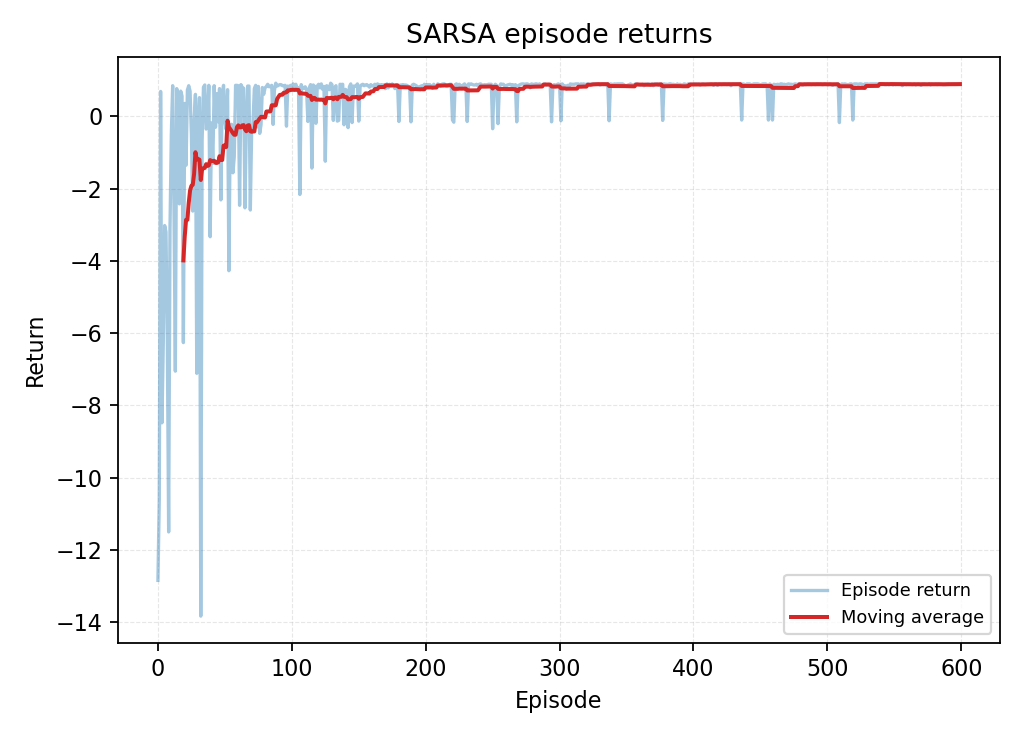
\includegraphics[width=0.8\linewidth]{sarsa_returns.png}
  \caption{SARSA episode returns showing convergence under \(\varepsilon\)-greedy policy}
  \label{fig:sarsa_returns}
\end{figure}

\begin{figure}[H]
  \centering
  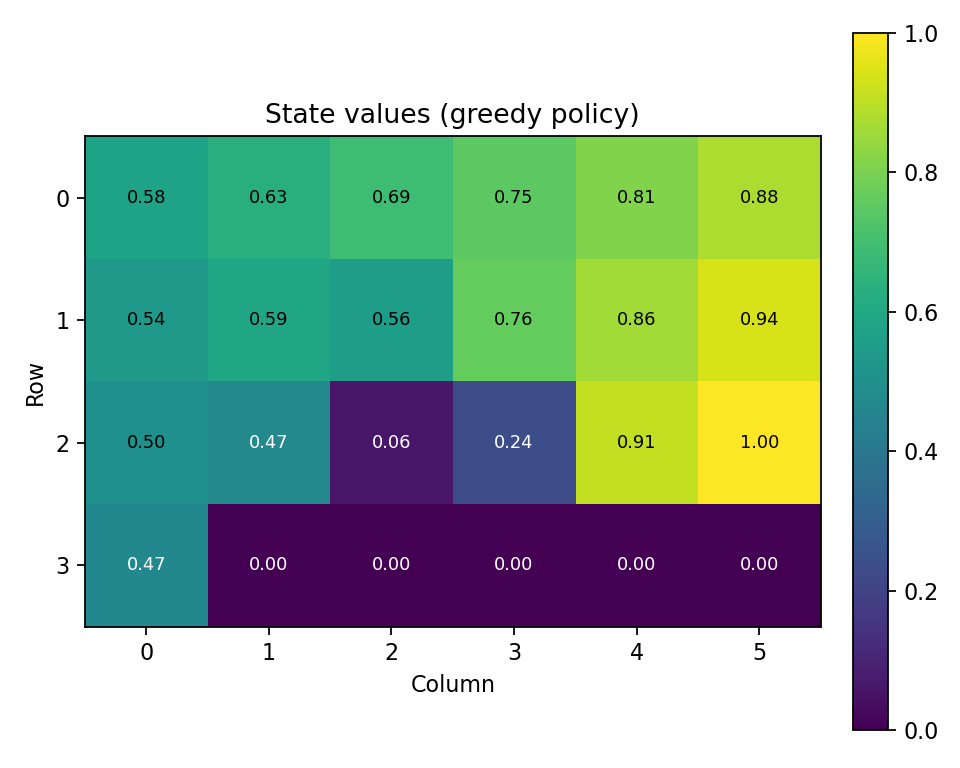
\includegraphics[width=0.82\linewidth]{sarsa_state_values.png}
  \caption{State-value heatmap reflecting the conservative policy learned near hazardous states}
  \label{fig:sarsa_state_values}
\end{figure}

\FloatBarrier
\section{Summary}
SARSA integrates exploration behaviour into its updates, yielding on-policy control well-suited for stochastic or risk-sensitive tasks. Proper tuning of learning rate and exploration schedule ensures stable convergence. The grid-world example highlights how returns stabilize and how the resulting value function captures safe routes.

\end{document}